\section{Постановка задачи}

\begin{frame}
    \frametitle{Постановка задачи}

    \begin{columns}

    \begin{column}{0.7\textwidth}
        \begin{figure}[H]
            \centering
            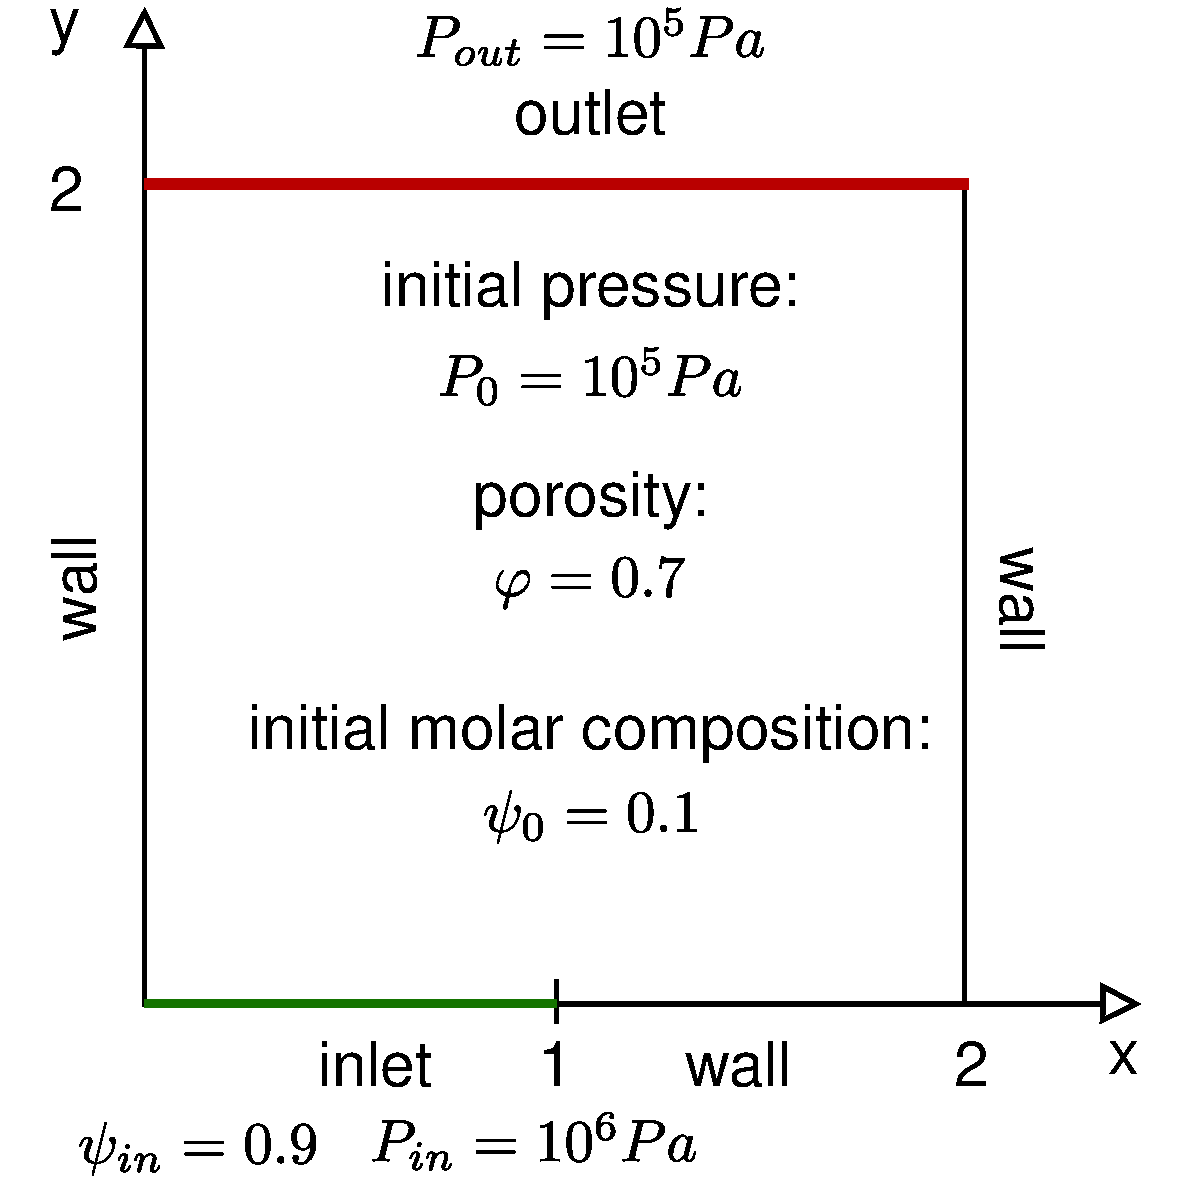
\includegraphics[height=0.8\textheight]
            {img/problem.pdf}
        \end{figure}
    \end{column}

    \begin{column}{0.4\textwidth}
        2-мерная задача:
        Моделирование фильтрации двухкомпонентной смеси 
        азота и пентана при предположении, что компоненты
        не смешиваются.
        Изотермическая задача.
    \end{column}

    \end{columns}

\end{frame}
